\section{Secondary 1K--100K Retrieval-Scale Study}
\subsection{Design}
To separate global-corpus growth from authorization-scope growth, we construct a deterministic nested master corpus of 100,000 Synthea patients. The original 1,000 patients remain the exact prefix. Additional records are deterministically selected and assigned so that each of A--D has either a fixed 200-patient ACL or a proportional ACL of 200, 2,000, and 20,000 at 1K, 10K, and 100K respectively; the protected share remains 20\% in the proportional condition.

A single TF-IDF(1,2) representation (float32) is fitted once on the 100K master and smaller conditions restrict candidate rows only. This avoids an IDF/vocabulary confound. Four hundred paired legitimate queries are evaluated per scale under unfiltered, fixed ACL, proportional ACL, and target-scoped controls. A 90-query LLM subset uses unfiltered, fixed-ACL, and target-fixed modes. Importantly, fixed-ACL and target-fixed candidate sets do not change with global scale; flat retrieval identity or answer behavior in those modes is therefore a \emph{construction control}, not an emergent scalability finding.

\subsection{Retrieval behavior}
Unfiltered median retrieval latency grows from 3.01 ms at 1K to 12.91 ms at 10K and 129.91 ms at 100K. The proportional ACL condition grows from 2.29 ms to 4.73 ms and 25.64 ms as its authorized candidate pool grows 200$\rightarrow$2,000$\rightarrow$20,000. The fixed 200-patient ACL condition remains near 2.3--2.8 ms because its candidate set is intentionally unchanged. The unfiltered 1K-vs-100K latency increase is significant under paired Wilcoxon testing ($p=2.73\times10^{-67}$); proportional-scope latency shows the same monotonic direction.

Distractor similarity also increases as the candidate pool grows. Median best-distractor TF-IDF similarity rises from 0.037 at 1K to 0.094 at 100K for unfiltered retrieval, and from 0.034 to 0.071 under proportional ACL. Correspondingly, the median target margin decreases from 0.322 to 0.264 unfiltered and from 0.329 to 0.289 proportional. Hit@1 remains 1.0 for these deliberately target-explicit legitimate queries, so the scale result is about increasing interference and cost, not target disappearance.

\begin{figure}[t]
\centering
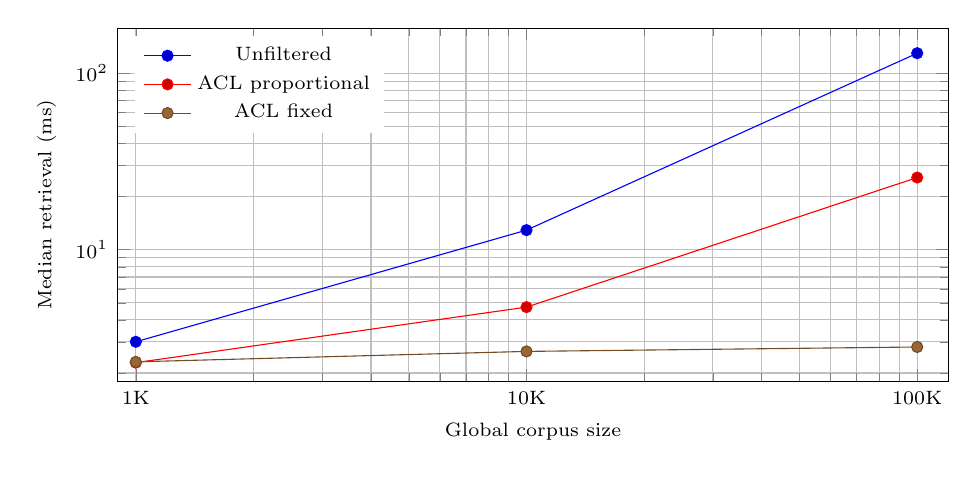
\begin{tikzpicture}
\begin{loglogaxis}[
  width=\columnwidth,height=0.50\columnwidth,
  xlabel={Global corpus size},ylabel={Median retrieval (ms)},
  xmin=900,xmax=120000,ymin=1.8,ymax=180,
  xtick={1000,10000,100000},xticklabels={1K,10K,100K},
  xticklabel style={font=\scriptsize},yticklabel style={font=\scriptsize},label style={font=\scriptsize},
  legend style={font=\scriptsize,draw=none,at={(0.02,0.98)},anchor=north west},
  grid=both]
\addplot+[mark=*] coordinates {(1000,3.0057) (10000,12.9066) (100000,129.9133)};
\addplot+[mark=*] coordinates {(1000,2.2896) (10000,4.7257) (100000,25.6390)};
\addplot+[mark=*] coordinates {(1000,2.3133) (10000,2.6512) (100000,2.8086)};
\legend{Unfiltered,ACL proportional,ACL fixed}
\end{loglogaxis}
\end{tikzpicture}
\caption{Median retrieval latency under nested scaling. Fixed ACL is a constant-candidate control; proportional ACL exposes the effect of growing authorization scope.}
\label{fig:scale_latency}
\end{figure}

\begin{table}[t]
\caption{Selected retrieval-scale outcomes (400 paired queries).}
\label{tab:scale}
\centering
\scriptsize
\begin{tabular}{lrrrr}
\toprule
Mode & Cand. 1K & Cand. 100K & Lat. 1K & Lat. 100K \\
\midrule
Unfiltered & 1,000 & 100,000 & 3.01 ms & 129.91 ms \\
ACL fixed & 200 & 200 & 2.31 ms & 2.81 ms \\
ACL proportional & 200 & 20,000 & 2.29 ms & 25.64 ms \\
Target fixed & 1 & 1 & 0.0006 ms & 0.0016 ms \\
\bottomrule
\end{tabular}
\end{table}

\subsection{LLM subset}
In the 90-query LLM subset, unfiltered \arsr{} is 68.9\% at 1K, 68.9\% at 10K, and 64.4\% at 100K. The paired 1K-vs-100K difference is not significant ($p=0.523$), so we do not claim generation-quality degradation from corpus growth. Target-fixed retrieval supplies the same one-record context by construction and yields 90.0\% at each scale; the unfiltered-vs-target-fixed difference is significant at each scale ($p=1.57\times10^{-4}$, $6.60\times10^{-5}$, and $5.65\times10^{-6}$). This demonstrates the utility of a target-scoped control for these queries, not scale-invariance as a discovered property. Fixed-ACL LLM retrieval likewise reuses the same 200 candidates and is not used to claim authorization-scope scaling.

\begin{figure}[t]
\centering
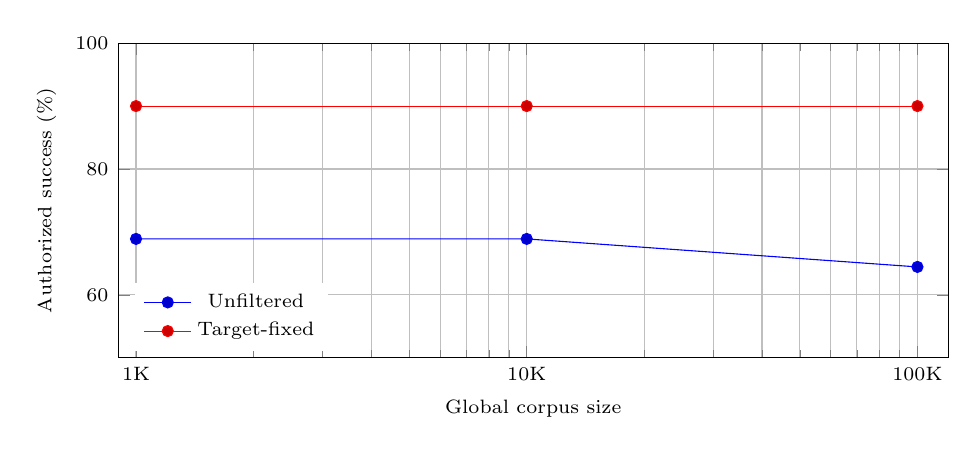
\begin{tikzpicture}
\begin{semilogxaxis}[
  width=\columnwidth,height=0.46\columnwidth,
  xlabel={Global corpus size},ylabel={Authorized success (\%)},
  xmin=900,xmax=120000,ymin=50,ymax=100,
  xtick={1000,10000,100000},xticklabels={1K,10K,100K},
  xticklabel style={font=\scriptsize},yticklabel style={font=\scriptsize},label style={font=\scriptsize},
  legend style={font=\scriptsize,draw=none,at={(0.02,0.02)},anchor=south west},
  grid=both]
\addplot+[mark=*] coordinates {(1000,68.89) (10000,68.89) (100000,64.44)};
\addplot+[mark=*] coordinates {(1000,90.0) (10000,90.0) (100000,90.0)};
\legend{Unfiltered,Target-fixed}
\end{semilogxaxis}
\end{tikzpicture}
\caption{LLM subset. Target-fixed provides a constant single-record context by construction; the unfiltered 1K-to-100K ARSR change is not significant.}
\label{fig:scale_llm}
\end{figure}

We intentionally do not make a generation-level claim for proportional ACL scope because that condition was evaluated only in the retrieval study. The 100K experiment is therefore a secondary systems result: it shows how candidate-set growth changes retrieval cost and interference, not whether authorization correctness depends on corpus size.
